In order to investigate the effectiveness of the human activity detection outdoors using our system, four different tasks were processed in the experiments. They were human recognition, human activity classification, people counting, and coarse-grained localization. As illustrated in Fig. \ref{fig_dia}, the output metric for human recognition is whether the target is human or animal, or there is no target. If the target is human, then the system further estimates whether the target is running or walking, how many people the target represents, and the rough range that the target is located in. Although the maximum number of people counted in a group is 4 and the ranges for rough localization are relatively narrow (only 2 meters apart because of the short detection range of the Bumblebee radar), it is foreseen that the methods used here could also be applied to a greater number of people and to radars that have greater detection ranges.

Three different experiments were performed in three different outdoor locations respectively. The experimental locations were populated with trees and shrubs; they were realistic wild areas. These experiments are described in detail below:  
\begin{figure}[!t]
\centering
%\captionsetup{justification=centering}
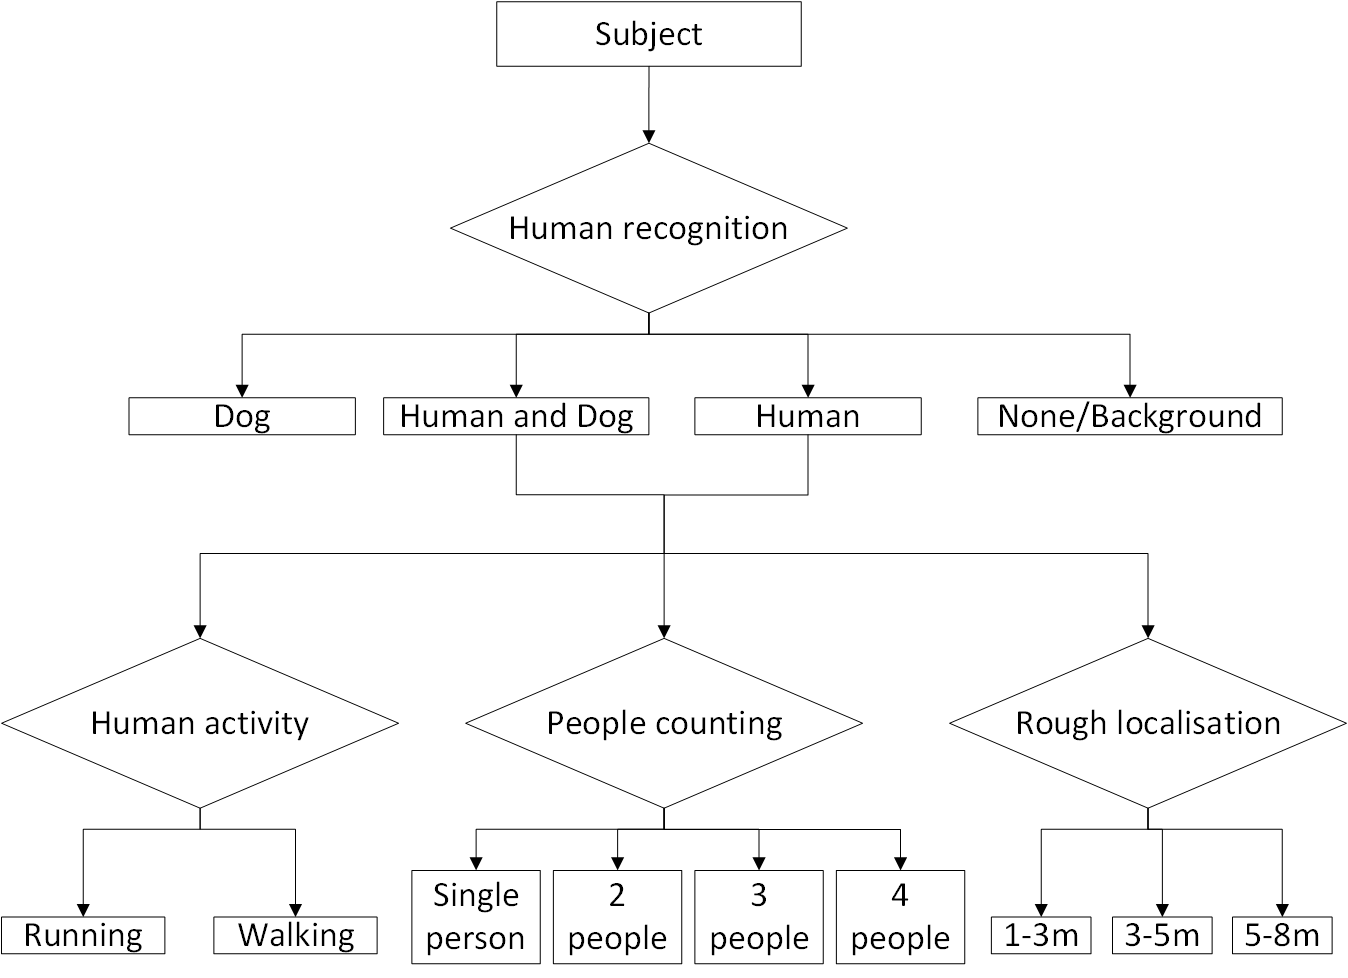
\includegraphics[width=3.5in]{diagram}
\caption{Workflow of four tasks, including human recognition, human activity \qquad detection, people counting, and coarse-grained localization}
\label{fig_dia}
\end{figure}

\textit{Case 1: Activity classification of a single person}: In this experiment, three individuals participated. Two types of activities (walking and running) were performed from three different angles ($\ang{0}$, $\ang{45}$, $\ang{90}$) relative to the radar beam. The same set of experiments was performed by each participant one at a time. At \ang{45} and \ang{90}, activities were performed in three different ranges, which were 1-3m, 3-5m, and 5-7m relative to the primary node. 

Fig. \ref{fig_mss} illustrates the micro-Doppler signatures of an individual participant walking at \ang{0}, \ang{45} and \ang{90}, which was collected by the radar system. The spectrograms were generated by a STFT with a sliding window size of 20s. As it can be seen, the spectrograms collected from outdoors are a little less clear than the ones collected indoors (as shown in Fig. 1). This is due to the complexity of the outdoor environment and a higher presence of noise. Comparing Fig. \ref{fig_mss}(a) and Fig. \ref{fig_mss}(b), the motion cycle of running is shorter than walking. There are more than three cycles in the spectrogram for running, but only 2 cycles in the spectrogram for walking. This confirms the physical fact that running takes less time to finish a motion cycle than walking. Another interesting finding is that the wave directions of Fig. \ref{fig_mss}(a) and Fig. \ref{fig_mss}(b) are opposite to the wave directions of Fig. \ref{fig_mss}(e) and Fig. \ref{fig_mss}(f), while the wave directions of Fig. \ref{fig_mss}(c) and Fig. \ref{fig_mss}(d) are the same as the Fig. \ref{fig_mss}(g) and Fig. \ref{fig_mss}(h). This is because the directions of the primary node and the secondary node are opposite to each other. When a person moves at \ang{0}, he/she is moving towards a radar and moving away from the other radar. The frequencies of the echoed wave signals of the two radars fluctuate in opposite directions. When a person moves at \ang{90} and \ang{45}, he/she gets close to or further away from both primary and second radars almost at the same time. The frequencies of the echoed wave signals of the two radars fluctuate in the same direction. Fig. \ref{fig_mss}(d) and Fig. \ref{fig_mss}(h) present more faded cycle segments, but in different positions. This is because when the participant is walking at \ang{45}, he/she is not within the detection range or he/she is at the edge of the range of each radar for a small period of time. In the spectrograms, the change in color intensity results from the changes in the radar cross-sections (RCS). The radar cross section (RCS) is the measure of a target's ability to reflect the radar signals in the direction of the radar's receiver, i.e. it is a measure of the ratio between the backscatter density in the direction of the radar (from the target) and the power density that is intercepted by the target. Larger RCS indicates a greater energy is reflected by the target, and it produces more intensive color in the spectrograms.
\begin{figure}[!t]
\centering
%\captionsetup{justification=centering}
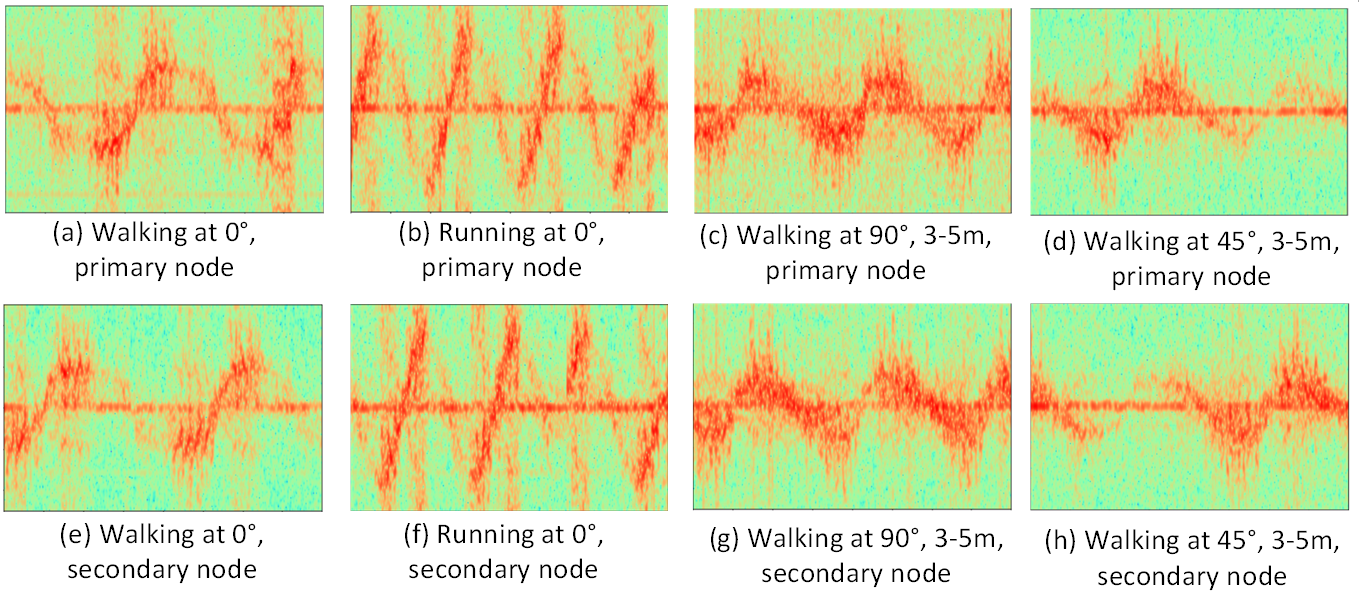
\includegraphics[width=3.7in]{ms_single}
\caption{Micro-Doppler signatures of an individual at different angles}
\label{fig_mss}
\end{figure}

The spectrograms in Fig. \ref{fig_ir9} represent the micro-Doppler signatures of an individual walking and running at \ang{90} in each one of the three ranges. As it can be seen, the patterns of the signal are different depending on the target’s distances to the primary node. The waveforms in Fig. \ref{fig_ir9}(a) and Fig. \ref{fig_ir9}(b) are smooth, the waveforms in Fig. \ref{fig_ir9}(c) and Fig. \ref{fig_ir9}(d) are more zigzagged, and the waveforms in Fig. \ref{fig_ir9}(e) and Fig. \ref{fig_ir9}(f) are discrete. The spectrograms of the secondary node are not shown, because the wave patterns collected by the secondary node in the range of 5-8m are similar to Fig. \ref{fig_ir9}(a) and Fig. \ref{fig_ir9}(b), the wave patterns in the range of 3-5m are similar to Fig. \ref{fig_ir9}(c) and Fig. \ref{fig_ir9}(d), and the wave patterns in the range of 1-3m are similar to Fig. \ref{fig_ir9}(e) and Fig. \ref{fig_ir9}(f). This indicates the distance does affect the wave pattern of the spectrograms of human activity.
\begin{figure}[!t]
\centering
%\captionsetup{justification=centering}
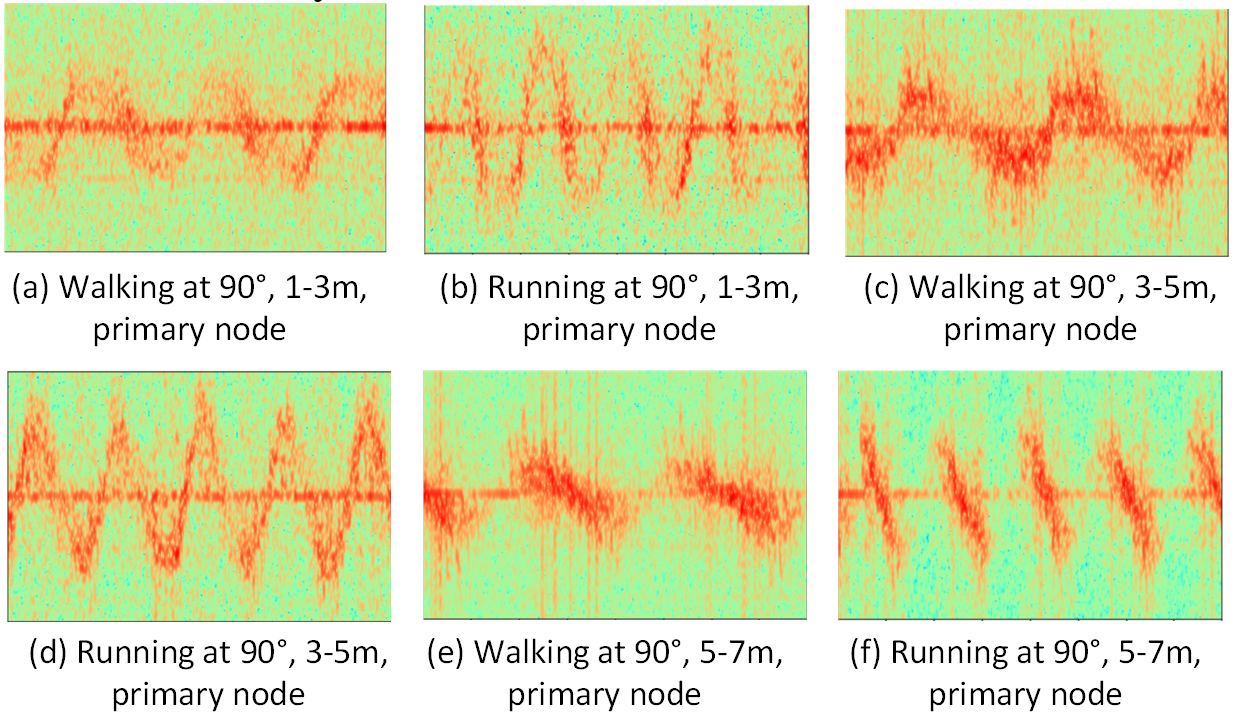
\includegraphics[width=3.5in]{individual_randar_90}
\caption{Micro-Doppler signatures of an individual walking and running in different ranges at \ang{90}}
\label{fig_ir9}
\end{figure}

Fig. \ref{fig_ir4} represents micro-Doppler signatures of an individual walking and running at \ang{45} in three different ranges. The patterns of these spectrograms are very similar to those of Fig.\ref{fig_ir9}, except that one part of each spectrogram is less clear, almost disappearing. This is because the target was not always in the detection range when he/she walked or ran back and forth at \ang{45}. Notice that the amplitude of the waves in Fig. \ref{fig_ir4} is a little smaller than in Fig. \ref{fig_ir9}.

\begin{figure}[!t]
\centering
%\captionsetup{justification=centering}
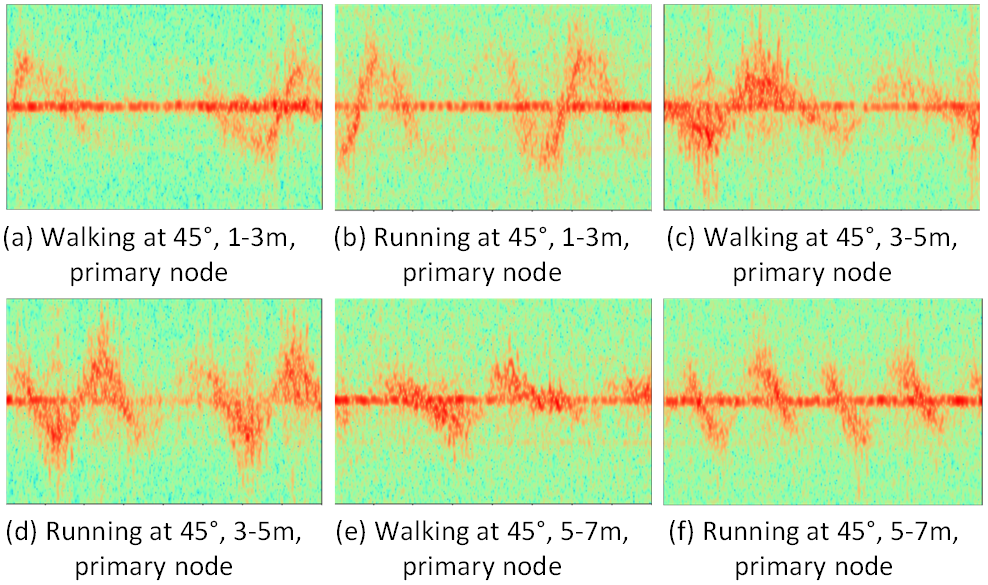
\includegraphics[width=3.5in]{individual_randar_45}
\caption{Micro-Doppler signatures of individual walking and running at \ang{45} with three different ranges}
\label{fig_ir4}
\end{figure}

\textit{Case 2: Activity classification and people counting in a group of people}: Nine individuals participated in this experiment, as shown in Fig. \ref{fig_ec}. Participants were arranged into three groups. The first group had two participants, the second group had three participants, and the third group consisted of four participants. Each group walked and ran in three ranges from three different angles (\ang{0}, \ang{45}, and \ang{90}) relative to the radar beam. Participants in the first or second group moved abreast. Participants in the third group were divided into two rows with two people in each row and they ran or walked at the same time inside the detection range. The main difference between \textit{Case 1} and \textit{Case 2} is the number of people that composed the target.
\begin{figure}[!t]
\centering
%\captionsetup{justification=centering}
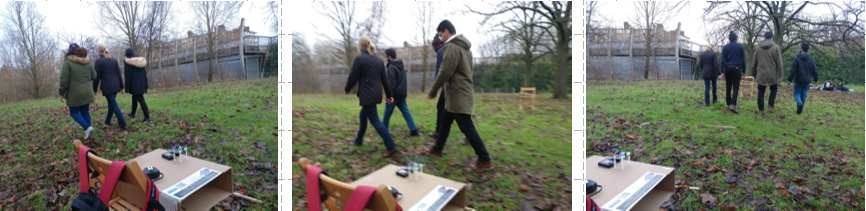
\includegraphics[width=3.5in]{ecounting}
\caption{Group behaviour classification and people counting}
\label{fig_ec}
\end{figure}

The spectrograms in Fig. \ref{fig_msc} show the micro-Doppler signatures of the target with different numbers of people. By the naked eye, it is difficult to find the visual differences among the spectrograms of different numbers of people. However, if we observe very carefully, it can be seen that the frequency waves in Fig. \ref{fig_msc}(c) and Fig. \ref{fig_msc}(d) are thicker than in Fig. \ref{fig_msc}(a) and Fig. \ref{fig_msc}(b). It could be understood that more people in a target would result in a more solid wave shape. However, this phenomenon cannot be observed in Fig. \ref{fig_msc}(e), Fig. \ref{fig_msc}(f), Fig. \ref{fig_msc}(g), and Fig. \ref{fig_msc}(h) possibly as a result of the speed of the movement. 
\begin{figure}[!t]
\centering
%\captionsetup{justification=centering}
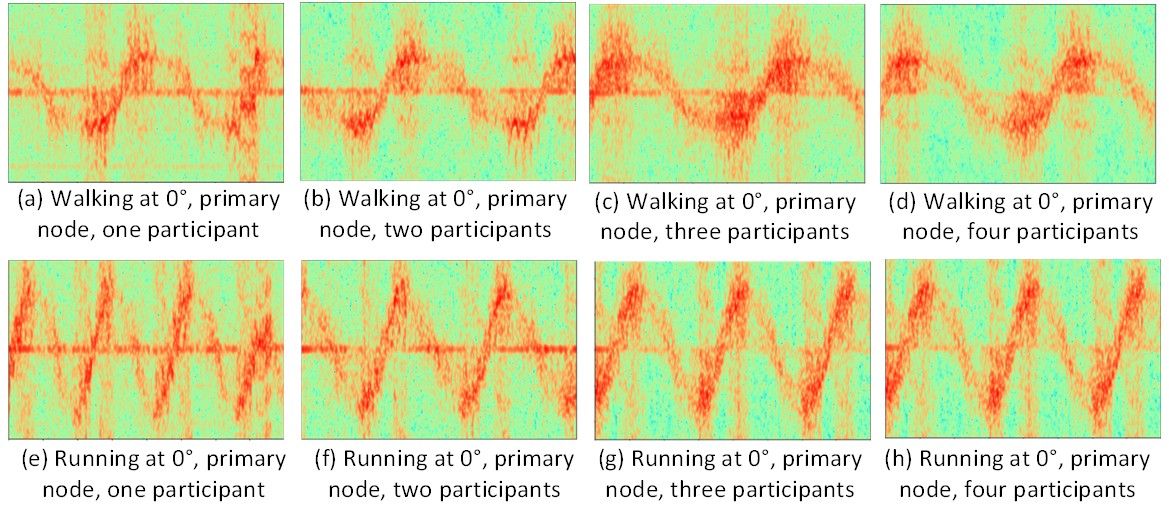
\includegraphics[width=3.7in]{mscounting}
\caption{Micro-Doppler signatures of different number of people}
\label{fig_msc}
\end{figure}

\textit{Case 3, differentiation between humans and dogs}: One human volunteer and two dogs participated in this experiment, as shown in Fig. \ref{fig_ani}. In the first experiment, separately, each dog was encouraged by their owners to move back and forth inside the detection range, in order to obtain micro-Doppler signatures of a dog only. In the second experiment, the volunteer walked a dog back and forth. Because it is hard to control the dog`’s speed (i.e. walk and run) inside the detection range, the experiment did not differentiate between walking and running, and only two angles (\ang{0} and \ang{90}) were investigated. Unavoidably, some noisy data was produced during the experiments, but the amount was small.  
\begin{figure}[!t]
\centering
%\captionsetup{justification=centering}
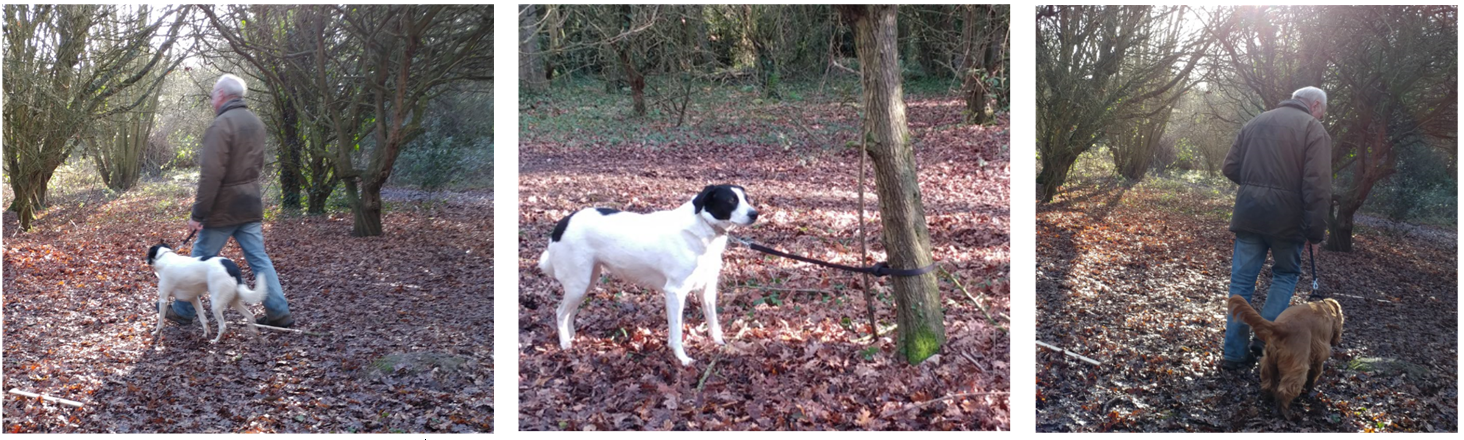
\includegraphics[width=3.6in]{animal}
\caption{Differentiation between humans and dogs}
\label{fig_ani}
\end{figure}

Combined with the data collected in \textit{Case 1} and \textit{Case 2}, all samples could be classified into 4 categories according to the different types of the targets, including human, dog, a person and a dog, and the background. As shown in Fig. \ref{fig_msani}, the spectrograms generated by different targets are different. Fig. \ref{fig_msani}(a) presents the periodic change of a human walking. Fig. \ref{fig_msani}(b) shows the micro-Doppler signatures of a moving dog. Visually, the frequency wave in Fig. \ref{fig_msani}(c) of a moving person and dog seems to have an overlapping shadow. The spectrogram of the scene background shown in Fig. \ref{fig_msani}(d) only contains a line around the frequency of 0Hz, this reflects the clutter in the environment around 0Hz. 
\begin{figure}[!t]
\centering
%\captionsetup{justification=centering}
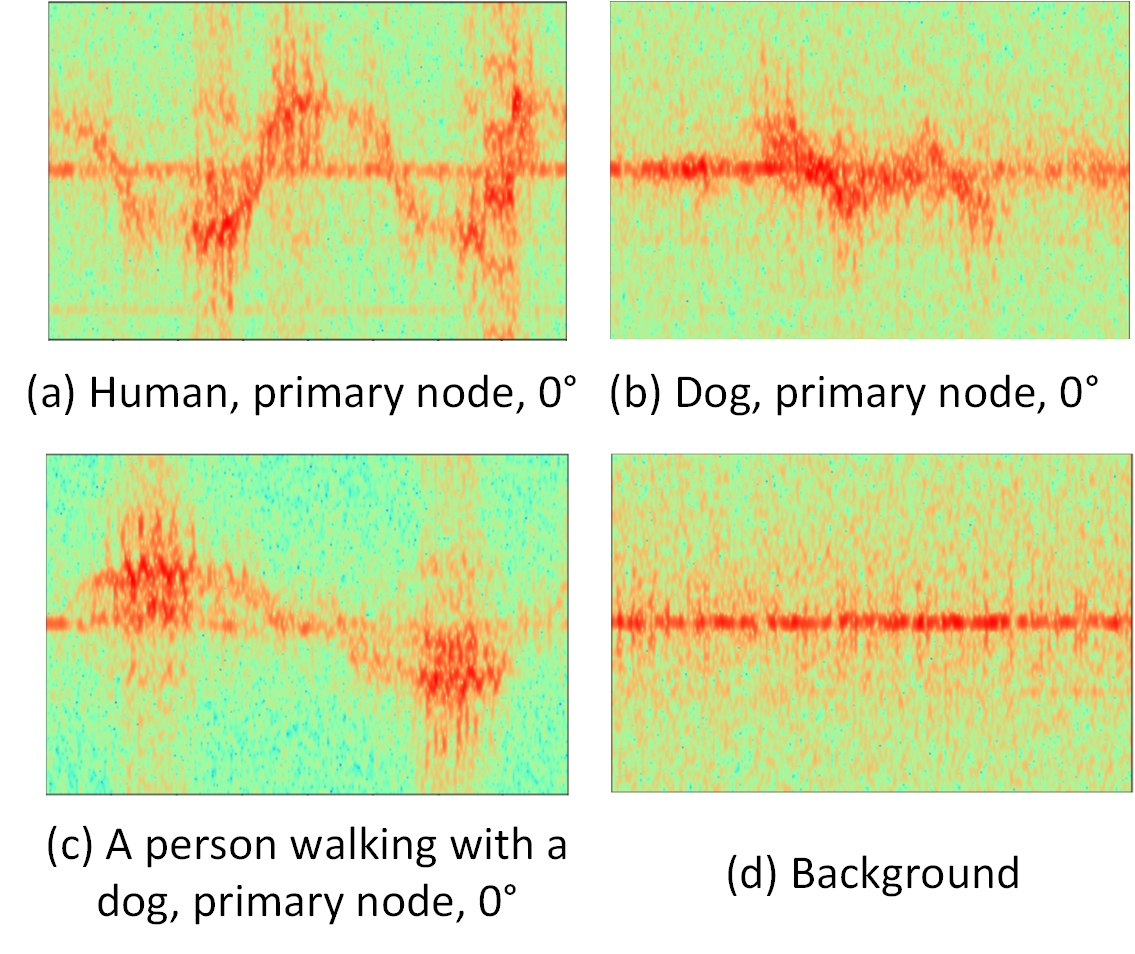
\includegraphics[width=3.4in]{msanimal}
\caption{Micro-Doppler signatures of different subjects}
\label{fig_msani}
\end{figure}